% !TeX root = ../main.tex
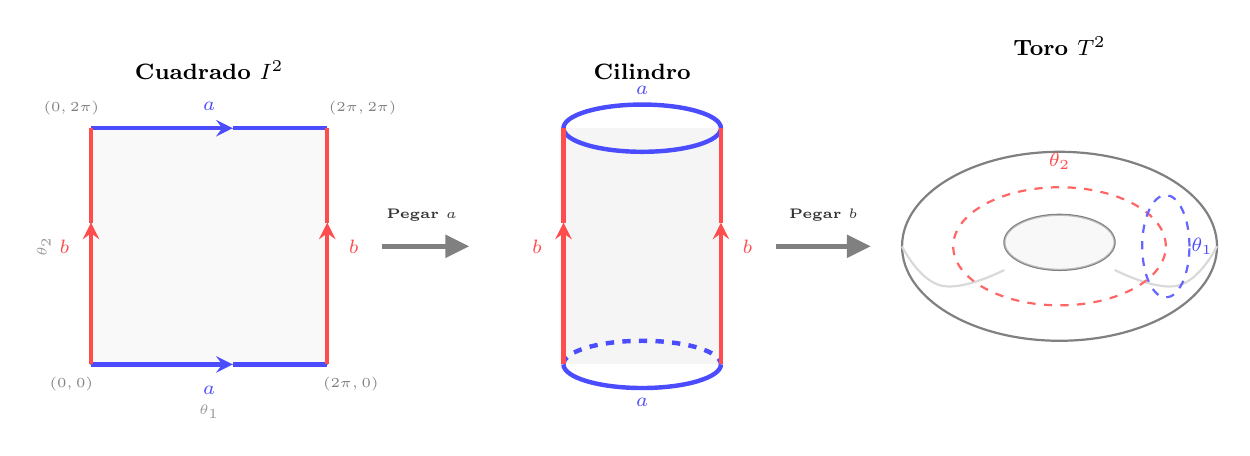
\begin{tikzpicture}[>=stealth, scale=1.0, every node/.style={font=\small}]

% =============================================
% PASO 1: Cuadrado unitario con identificaciones
% =============================================
\begin{scope}[shift={(-5.5,0)}]
    \node[anchor=south, font=\bfseries\footnotesize] at (1.5, 3.5) {Cuadrado $I^2$};
    
    % Cuadrado
    \fill[gray!5] (0,0) rectangle (3,3);
    \draw[black!40, thin] (0,0) rectangle (3,3);
    
    % Borde inferior (flecha a la derecha, azul)
    \draw[blue!70, ultra thick, ->] (0,0) -- (1.8,0);
    \draw[blue!70, ultra thick] (1.8,0) -- (3,0);
    \node[font=\scriptsize, blue!70, anchor=north] at (1.5,-0.15) {$a$};
    
    % Borde superior (flecha a la derecha, azul — mismo sentido = se pegan)
    \draw[blue!70, ultra thick, ->] (0,3) -- (1.8,3);
    \draw[blue!70, ultra thick] (1.8,3) -- (3,3);
    \node[font=\scriptsize, blue!70, anchor=south] at (1.5,3.1) {$a$};
    
    % Borde izquierdo (flecha hacia arriba, rojo)
    \draw[red!70, ultra thick, ->] (0,0) -- (0,1.8);
    \draw[red!70, ultra thick] (0,1.8) -- (0,3);
    \node[font=\scriptsize, red!70, anchor=east] at (-0.15,1.5) {$b$};
    
    % Borde derecho (flecha hacia arriba, rojo — mismo sentido = se pegan)
    \draw[red!70, ultra thick, ->] (3,0) -- (3,1.8);
    \draw[red!70, ultra thick] (3,1.8) -- (3,3);
    \node[font=\scriptsize, red!70, anchor=west] at (3.15,1.5) {$b$};
    
    % Etiquetas de esquinas
    \node[font=\tiny, black!50] at (-0.25,-0.25) {$(0,0)$};
    \node[font=\tiny, black!50] at (3.3,-0.25) {$(2\pi,0)$};
    \node[font=\tiny, black!50] at (-0.25,3.25) {$(0,2\pi)$};
    \node[font=\tiny, black!50] at (3.45,3.25) {$(2\pi,2\pi)$};
    
    % Ejes dentro del cuadrado
    \node[font=\tiny\bfseries, gray!80] at (1.5,-0.6) {$\theta_1$};
    \node[font=\tiny\bfseries, gray!80, rotate=90] at (-0.6,1.5) {$\theta_2$};
\end{scope}

% =============================================
% FLECHA: Paso 1 → Paso 2
% =============================================
\draw[ultra thick, black!50] (-1.8,1.5) -- (-0.9,1.5); % La línea termina un poco antes
\fill[black!50] (-0.7,1.5) -- (-1.0,1.65) -- (-1.0,1.35) -- cycle; % Dibujamos el triángulo
\node[anchor=south, font=\tiny\bfseries, black!80] at (-1.3,1.7) {Pegar $a$};

% =============================================
% PASO 2: Cilindro (bordes azules pegados)
% =============================================
\begin{scope}[shift={(0.5,0)}]
    \node[anchor=south, font=\bfseries\footnotesize] at (1, 3.5) {Cilindro};
    
    % Cuerpo del cilindro
    \fill[gray!8] (0,0) -- (2,0) -- (2,3) -- (0,3) -- cycle;
    
    % BORDE SUPERIOR (Borde 'a' pegado)
    % Lo dibujamos en azul ultra thick para indicar que es la unión de los bordes 'a'
    \draw[blue!70, ultra thick] (1,3) ellipse (1 and 0.3);
    \node[font=\scriptsize, blue!70, anchor=south] at (1,3.3) {$a$};
    
    % BORDE INFERIOR (Borde 'a' pegado)
    % Parte de atrás punteada, parte de adelante sólida y azul
    \draw[blue!70, ultra thick, dashed] (0,0) arc[start angle=180, end angle=0, x radius=1, y radius=0.3];
    \draw[blue!70, ultra thick] (0,0) arc[start angle=180, end angle=360, x radius=1, y radius=0.3];
    \node[font=\scriptsize, blue!70, anchor=north] at (1,-0.3) {$a$};
    
    % Lados del cilindro (Bordes 'b' rojos)
    \draw[red!70, ultra thick, ->] (0,0) -- (0,1.8);
    \draw[red!70, ultra thick] (0,1.8) -- (0,3);
    \node[font=\scriptsize, red!70, anchor=east] at (-0.15,1.5) {$b$};
    
    \draw[red!70, ultra thick, ->] (2,0) -- (2,1.8);
    \draw[red!70, ultra thick] (2,1.8) -- (2,3);
    \node[font=\scriptsize, red!70, anchor=west] at (2.15,1.5) {$b$};
\end{scope}
% =============================================
% FLECHA: Paso 2 → Paso 3
% =============================================
% 1. La línea (termina en 4.2 en lugar de 4.4 para dejar espacio al triángulo)
\draw[ultra thick, black!50] (3.2,1.5) -- (4.2,1.5);
% Coordenadas: (Punta), (Esquina superior atrás), (Esquina inferior atrás)
\fill[black!50] (4.4, 1.5) -- (4.1, 1.65) -- (4.1, 1.35) -- cycle;
\node[anchor=south, font=\tiny\bfseries, black!80] at (3.8,1.7) {Pegar $b$};

% =============================================
% PASO 3: Toro T² (dona)
% =============================================
\begin{scope}[shift={(6.8,1.5)}]
    \node[anchor=south, font=\bfseries\footnotesize] at (0, 2.3) {Toro $T^2$};
    
    % Toro exterior
    \draw[black!50, thick] (0,0) ellipse (2 and 1.2);
    
    % Agujero del toro
    \draw[black!50, thick] (0,0.05) ellipse (0.7 and 0.35);
    
    % Curvas de profundidad
    \draw[gray!30, thick] 
        plot[smooth, tension=0.8] coordinates {(-2,0) (-1.5,-0.5) (-0.7,-0.3)};
    \draw[gray!30, thick] 
        plot[smooth, tension=0.8] coordinates {(0.7,-0.3) (1.5,-0.5) (2,0)};
    
    \fill[gray!10, opacity=0.5] (0,0.05) ellipse (0.7 and 0.35);
    
    % --- EL CAMBIO ESTÁ AQUÍ ---
    
    % θ₂: Ahora es el círculo GRANDE (azul) que recorre la dona
    % Porque viene del eje vertical que se estiró al cerrar el cilindro
    \draw[red!60, thick, dashed] (0,0) ellipse (1.35 and 0.75);
    \node[font=\scriptsize, red!70, anchor=south] at (0,0.85) {$\theta_2$};
    
    % θ₁: Ahora es el círculo PEQUEÑO (azul) que es la sección del cilindro
    % Es el que se formó al "pegar a"
    \draw[blue!60, thick, dashed] (1.35,0) ellipse (0.3 and 0.65);
    \node[font=\scriptsize, blue!70, anchor=west] at (1.55,0) {$\theta_1$};
\end{scope}

\end{tikzpicture}
